\documentclass{article}

\usepackage{amssymb, amsmath, amsthm, tikz, verbatim, graphicx,lmodern,indentfirst,enumerate,color}

\usepackage[titletoc,page]{appendix}
\usepackage[margin=1.4in]{geometry}

\newtheorem{thm}{Theorem}[section]
\newtheorem{lem}[thm]{Lemma}
\newtheorem{prop}[thm]{Proposition}
\newtheorem{cor}[thm]{Corollary}
\newtheorem{con}[thm]{Conjecture}
\newtheorem{oprob}[thm]{Open Problem}
\newtheorem{prob}[thm]{Problem}

\theoremstyle{definition}
\newtheorem{example}[thm]{Example}

\theoremstyle{definition}
\newtheorem{question}[thm]{Question}

\theoremstyle{definition}
\newtheorem{defn}[thm]{Definition}

\theoremstyle{remark}
\newtheorem{rem}[thm]{Remark}

\numberwithin{equation}{section}

\newcommand*\circled[1]{\tikz[baseline=(char.base)]{
            \node[shape=circle,draw,inner sep=0pt,minimum size=5mm] (char) {#1};}}
\newcommand*\circleD[1]{\tikz[baseline=(char.base)]{
            \node[shape=circle,draw,inner sep=0pt,minimum size=7mm] (char) {#1};}}

\newcommand{\rootsG}[8]{\circled{#1}
            \begin{tabular}{cccccc}
             &&&#2&& \\
             #3&#4&#5&#6&#7&#8
             \end{tabular}}
\newcommand{\rootsE}[7]{\circled{#1}
            \begin{tabular}{ccccc}
             &&#2&& \\
             #3&#4&#5&#6&#7
             \end{tabular}}
\newcommand{\rootsC}[9]{\circleD{#1}
            \begin{tabular}{ccccccc}
             &&&&#2&& \\
             #3&#4&#5&#6&#7&#8&#9
             \end{tabular}}
\newcommand{\rootsD}[5]{\circled{#1}
            \begin{tabular}{ccc}
             &#2& \\
             #3&#4&#5
             \end{tabular}}
\makeatletter
\newcommand{\rmnum}[1]{\romannumeral #1}
\newcommand{\Rmnum}[1]{\expandafter\@slowromancap\romannumeral #1@}
\makeatother
\bibliographystyle{plain}
\begin{document}

\documentclass{article}

\usepackage{authblk}
\usepackage{orcidlink}

\title{A Relationship Between Spin and Geometry}
\author{Peter T. J. Bradshaw\,\orcidlink{0000-0001-9938-8460}\thanks{ucapptj@ucl.ac.uk, orcid.org/0000-0001-9938-8460}}
\affil{\textit{Department of Physics and Astronomy, University College London, London, WC1E 6BT}}
\date{}

\begin{document}
\maketitle
\end{document}

\IEEEraisesectionheading{\section{Introduction}}

\IEEEPARstart{V}{ision} system is studied in orthogonal disciplines spanning from neurophysiology and psychophysics to computer science all with uniform objective: understand the vision system and develop it into an integrated theory of vision. In general, vision or visual perception is the ability of information acquisition from environment, and it's interpretation. According to Gestalt theory, visual elements are perceived as patterns of wholes rather than the sum of constituent parts~\cite{koffka2013principles}. The Gestalt theory through \textit{emergence}, \textit{invariance}, \textit{multistability}, and \textit{reification} properties (aka Gestalt principles), describes how vision recognizes an object as a \textit{whole} from constituent parts. There is an increasing interested to model the cognitive aptitude of visual perception; however, the process is challenging. In the following, a challenge (as an example) per object and motion perception is discussed. 



\subsection{Why do things look as they do?}
In addition to Gestalt principles, an object is characterized with its spatial parameters and material properties. Despite of the novel approaches proposed for material recognition (e.g.,~\cite{sharan2013recognizing}), objects tend to get the attention. Leveraging on an object's spatial properties, material, illumination, and background; the mapping from real world 3D patterns (distal stimulus) to 2D patterns onto retina (proximal stimulus) is many-to-one non-uniquely-invertible mapping~\cite{dicarlo2007untangling,horn1986robot}. There have been novel biology-driven studies for constructing computational models to emulate anatomy and physiology of the brain for real world object recognition (e.g.,~\cite{lowe2004distinctive,serre2007robust,zhang2006svm}), and some studies lead to impressive accuracy. For instance, testing such computational models on gold standard controlled shape sets such as Caltech101 and Caltech256, some methods resulted $<$60\% true-positives~\cite{zhang2006svm,lazebnik2006beyond,mutch2006multiclass,wang2006using}. However, Pinto et al.~\cite{pinto2008real} raised a caution against the pervasiveness of such shape sets by highlighting the unsystematic variations in objects features such as spatial aspects, both between and within object categories. For instance, using a V1-like model (a neuroscientist's null model) with two categories of systematically variant objects, a rapid derogate of performance to 50\% (chance level) is observed~\cite{zhang2006svm}. This observation accentuates the challenges that the infinite number of 2D shapes casted on retina from 3D objects introduces to object recognition. 

Material recognition of an object requires in-depth features to be determined. A mineralogist may describe the luster (i.e., optical quality of the surface) with a vocabulary like greasy, pearly, vitreous, resinous or submetallic; he may describe rocks and minerals with their typical forms such as acicular, dendritic, porous, nodular, or oolitic. We perceive materials from early age even though many of us lack such a rich visual vocabulary as formalized as the mineralogists~\cite{adelson2001seeing}. However, methodizing material perception can be far from trivial. For instance, consider a chrome sphere with every pixel having a correspondence in the environment; hence, the material of the sphere is hidden and shall be inferred implicitly~\cite{shafer2000color,adelson2001seeing}. Therefore, considering object material, object recognition requires surface reflectance, various light sources, and observer's point-of-view to be taken into consideration.


\subsection{What went where?}
Motion is an important aspect in interpreting the interaction with subjects, making the visual perception of movement a critical cognitive ability that helps us with complex tasks such as discriminating moving objects from background, or depth perception by motion parallax. Cognitive susceptibility enables the inference of 2D/3D motion from a sequence of 2D shapes (e.g., movies~\cite{niyogi1994analyzing,little1998recognizing,hayfron2003automatic}), or from a single image frame (e.g., the pose of an athlete runner~\cite{wang2013learning,ramanan2006learning}). However, its challenging to model the susceptibility because of many-to-one relation between distal and proximal stimulus, which makes the local measurements of proximal stimulus inadequate to reason the proper global interpretation. One of the various challenges is called \textit{motion correspondence problem}~\cite{attneave1974apparent,ullman1979interpretation,ramachandran1986perception,dawson1991and}, which refers to recognition of any individual component of proximal stimulus in frame-1 and another component in frame-2 as constituting different glimpses of the same moving component. If one-to-one mapping is intended, $n!$ correspondence matches between $n$ components of two frames exist, which is increased to $2^n$  for one-to-any mappings. To address the challenge, Ullman~\cite{ullman1979interpretation} proposed a method based on nearest neighbor principle, and Dawson~\cite{dawson1991and} introduced an auto associative network model. Dawson's network model~\cite{dawson1991and} iteratively modifies the activation pattern of local measurements to achieve a stable global interpretation. In general, his model applies three constraints as it follows
\begin{inlinelist}
	\item \textit{nearest neighbor principle} (shorter motion correspondence matches are assigned lower costs)
	\item \textit{relative velocity principle} (differences between two motion correspondence matches)
	\item \textit{element integrity principle} (physical coherence of surfaces)
\end{inlinelist}.
According to experimental evaluations (e.g.,~\cite{ullman1979interpretation,ramachandran1986perception,cutting1982minimum}), these three constraints are the aspects of how human visual system solves the motion correspondence problem. Eom et al.~\cite{eom2012heuristic} tackled the motion correspondence problem by considering the relative velocity and the element integrity principles. They studied one-to-any mapping between elements of corresponding fuzzy clusters of two consecutive frames. They have obtained a ranked list of all possible mappings by performing a state-space search. 



\subsection{How a stimuli is recognized in the environment?}

Human subjects are often able to recognize a 3D object from its 2D projections in different orientations~\cite{bartoshuk1960mental}. A common hypothesis for this \textit{spatial ability} is that, an object is represented in memory in its canonical orientation, and a \textit{mental rotation} transformation is applied on the input image, and the transformed image is compared with the object in its canonical orientation~\cite{bartoshuk1960mental}. The time to determine whether two projections portray the same 3D object
\begin{inlinelist}
	\item increase linearly with respect to the angular disparity~\cite{bartoshuk1960mental,cooperau1973time,cooper1976demonstration}
	\item is independent from the complexity of the 3D object~\cite{cooper1973chronometric}
\end{inlinelist}.
Shepard and Metzler~\cite{shepard1971mental} interpreted this finding as it follows: \textit{human subjects mentally rotate one portray at a constant speed until it is aligned with the other portray.}



\subsection{State of the Art}

The linear mapping transformation determination between two objects is generalized as determining optimal linear transformation matrix for a set of observed vectors, which is first proposed by Grace Wahba in 1965~\cite{wahba1965least} as it follows. 
\textit{Given two sets of $n$ points $\{v_1, v_2, \dots v_n\}$, and $\{v_1^*, v_2^* \dots v_n^*\}$, where $n \geq 2$, find the rotation matrix $M$ (i.e., the orthogonal matrix with determinant +1) which brings the first set into the best least squares coincidence with the second. That is, find $M$ matrix which minimizes}
\begin{equation}
	\sum_{j=1}^{n} \vert v_j^* - Mv_j \vert^2
\end{equation}

Multiple solutions for the \textit{Wahba's problem} have been published, such as Paul Davenport's q-method. Some notable algorithms after Davenport's q-method were published; of that QUaternion ESTimator (QU\-EST)~\cite{shuster2012three}, Fast Optimal Attitude Matrix \-(FOAM)~\cite{markley1993attitude} and Slower Optimal Matrix Algorithm (SOMA)~\cite{markley1993attitude}, and singular value decomposition (SVD) based algorithms, such as Markley’s SVD-based method~\cite{markley1988attitude}. 

In statistical shape analysis, the linear mapping transformation determination challenge is studied as Procrustes problem. Procrustes analysis finds a transformation matrix that maps two input shapes closest possible on each other. Solutions for Procrustes problem are reviewed in~\cite{gower2004procrustes,viklands2006algorithms}. For orthogonal Procrustes problem, Wolfgang Kabsch proposed a SVD-based method~\cite{kabsch1976solution} by minimizing the root mean squared deviation of two input sets when the determinant of rotation matrix is $1$. In addition to Kabsch’s partial Procrustes superimposition (covers translation and rotation), other full Procrustes superimpositions (covers translation, uniform scaling, rotation/reflection) have been proposed~\cite{gower2004procrustes,viklands2006algorithms}. The determination of optimal linear mapping transformation matrix using different approaches of Procrustes analysis has wide range of applications, spanning from forging human hand mimics in anthropomorphic robotic hand~\cite{xu2012design}, to the assessment of two-dimensional perimeter spread models such as fire~\cite{duff2012procrustes}, and the analysis of MRI scans in brain morphology studies~\cite{martin2013correlation}.

\subsection{Our Contribution}

The present study methodizes the aforementioned mentioned cognitive susceptibilities into a cognitive-driven linear mapping transformation determination algorithm. The method leverages on mental rotation cognitive stages~\cite{johnson1990speed} which are defined as it follows
\begin{inlinelist}
	\item a mental image of the object is created
	\item object is mentally rotated until a comparison is made
	\item objects are assessed whether they are the same
	\item the decision is reported
\end{inlinelist}.
Accordingly, the proposed method creates hierarchical abstractions of shapes~\cite{greene2009briefest} with increasing level of details~\cite{konkle2010scene}. The abstractions are presented in a vector space. A graph of linear transformations is created by circular-shift permutations (i.e., rotation superimposition) of vectors. The graph is then hierarchically traversed for closest mapping linear transformation determination. 

Despite of numerous novel algorithms to calculate linear mapping transformation, such as those proposed for Procrustes analysis, the novelty of the presented method is being a cognitive-driven approach. This method augments promising discoveries on motion/object perception into a linear mapping transformation determination algorithm.



\section{Preliminaries}
Throughout, we denote by $k$ a separably closed field. Our references for algebraic groups are~\cite{Borel-AG-book},~\cite{Borel-Tits-Groupes-reductifs},~\cite{Conrad-pred-book},~\cite{Humphreys-book1}, and~\cite{Springer-book}. 

Let $H$ be a (possibly non-connected) affine algebraic group. We write $H^{\circ}$ for the identity component of $H$. We write $[H,H]$ for the derived group of $H$. A reductive group $G$ is called \emph{simple} as an algebraic group if $G$ is connected and all proper normal subgroups of $G$ are finite. We write $X_k(G)$ and $Y_k(G)$ ($X(G)$ and $Y(G)$) for the set of $k$-characters and $k$-cocharacters ($\overline k$-characters and $\overline k$-cocharacters) of $G$ respectively. For $\overline k$-characters and $\overline k$-cocharacters $G$ we simply say characters and cocharacters of $G$. 

Fix a maximal $k$-torus $T$ of $G$ (such a $T$ exists by~\cite[Cor.~18.8]{Borel-AG-book}). Then $T$ splits over $k$ since $k$ is separably closed. Let $\Psi(G,T)$ denote the set of roots of $G$ with respect to $T$. We sometimes write $\Psi(G)$ for $\Psi(G,T)$. Let $\zeta\in\Psi(G)$. We write $U_\zeta$ for the corresponding root subgroup of $G$. We define $G_\zeta := \langle U_\zeta, U_{-\zeta} \rangle$. Let $\zeta, \xi \in \Psi(G)$. Let $\xi^{\vee}$ be the coroot corresponding to $\xi$. Then $\zeta\circ\xi^{\vee}:\overline k^{*}\rightarrow \overline k^{*}$ is a $k$-homomorphism such that $(\zeta\circ\xi^{\vee})(a) = a^n$ for some $n\in\mathbb{Z}$.
Let $s_\xi$ denote the reflection corresponding to $\xi$ in the Weyl group of $G$. Each $s_\xi$ acts on the set of roots $\Psi(G)$ by the following formula~\cite[Lem.~7.1.8]{Springer-book}:
$
s_\xi\cdot\zeta = \zeta - \langle \zeta, \xi^{\vee} \rangle \xi. 
$
\noindent By \cite[Prop.~6.4.2, Lem.~7.2.1]{Carter-simple-book} we can choose $k$-homomorphisms $\epsilon_\zeta : \overline k \rightarrow U_\zeta$  so that 
$
n_\xi \epsilon_\zeta(a) n_\xi^{-1}= \epsilon_{s_\xi\cdot\zeta}(\pm a)
            \text{ where } n_\xi = \epsilon_\xi(1)\epsilon_{-\xi}(-1)\epsilon_{\xi}(1).  \label{n-action on group}
$




The next result~\cite[Prop.~1.12]{Uchiyama-Nonperfect-pre} shows complete reducibility behaves nicely under central isogenies. In this paper we do not specify the isogeny type of $G$. (Our argument works for $G$ of any isogeny type anyway.) Note that if $k$ is algebraically closed, the centrality assumption for $f$ is not necessary in Proposition~\ref{isogeny}. 
\begin{defn}
Let $G_1$ and $G_2$ be reductive $k$-groups. A $k$-isogeny $f:G_1\rightarrow G_2$ is \emph{central} if $\textup{ker}\,df_1$ is central in $\mathfrak{g_1}$ where $\textup{ker}\,df_1$ is the differential of $f$ at the identity of $G_1$ and $\mathfrak{g_1}$ is the Lie algebra of $G_1$. 
\end{defn}
\begin{prop}\label{isogeny}
Let $G_1$ and $G_2$ be reductive $k$-groups. Let $H_1$ and $H_2$ be subgroups of $G_1$ and $G_2$ be subgroups of $G_1$ and $G_2$ respectively. Let $f:G_1 \rightarrow G_2$ be a central $k$-isogeny. 
\begin{enumerate}
\item{If $H_1$ is $G_1$-cr over $k$, then $f(H_1)$ is $G_2$-cr over $k$.}
\item{If $H_2$ is $G_2$-cr over $k$, then $f^{-1}(H_2)$ is $G_1$-cr over $k$.} 
\end{enumerate}
\end{prop}


The next result~\cite[Thm.~1.4]{Bate-cocharacterbuildings-Arx} is used repeatedly to reduce problems on $G$-complete reducibility to those on $L$-complete reducibility where $L$ is a Levi subgroup of $G$. 

\begin{prop}\label{G-cr-L-cr}
Suppose that a subgroup $H$ of $G$ is contained in a $k$-defined Levi subgroup of $G$. Then $H$ is $G$-cr over $k$ if and only if it is $L$-cr over $k$. 
\end{prop}


We recall characterizations of parabolic subgroups, Levi subgroups, and unipotent radicals in terms of cocharacters of $G$~\cite[Prop.~8.4.5]{Springer-book}. These characterizations are essential to translate results on complete reducibility into the language of GIT; see~\cite{Bate-geometric-Inventione},~\cite{Bate-uniform-TransAMS} for example. 

\begin{defn}
Let $X$ be a affine $k$-variety. Let $\phi : \overline k^*\rightarrow X$ be a $k$-morphism of affine $k$-varieties. We say that $\displaystyle\lim_{a\rightarrow 0}\phi(a)$ exists if there exists a $k$-morphism $\hat\phi:\overline k\rightarrow X$ (necessarily unique) whose restriction to $\overline k^{*}$ is $\phi$. If this limit exists, we set $\displaystyle\lim_{a\rightarrow 0}\phi(a) = \hat\phi(0)$.
\end{defn}

\begin{defn}\label{R-parabolic}
Let $\lambda\in Y(G)$. Define
$
P_\lambda := \{ g\in G \mid \displaystyle\lim_{a\rightarrow 0}\lambda(a)g\lambda(a)^{-1} \text{ exists}\}, $\\
$L_\lambda := \{ g\in G \mid \displaystyle\lim_{a\rightarrow 0}\lambda(a)g\lambda(a)^{-1} = g\}, \,
R_u(P_\lambda) := \{ g\in G \mid  \displaystyle\lim_{a\rightarrow0}\lambda(a)g\lambda(a)^{-1} = 1\}. 
$
\end{defn}
Then $P_\lambda$ is a parabolic subgroup of $G$, $L_\lambda$ is a Levi subgroup of $P_\lambda$, and $R_u(P_\lambda)$ is the unipotent radical of $P_\lambda$. If $\lambda$ is $k$-defined, $P_\lambda$, $L_\lambda$, and $R_u(P_\lambda)$ are $k$-defined~\cite[Sec.~2.1-2.3]{Richardson-conjugacy-Duke}. Any $k$-defined parabolic subgroups and $k$-defined Levi subgroups of $G$ arise in this way since $k$ is separably closed. It is well known that $L_\lambda = C_G(\lambda(\overline k^*))$. Note that $k$-defined Levi subgroups of a $k$-defined parabolic subgroup $P$ of $G$ are $R_u(P)(k)$-conjugate~\cite[Lem.~2.5(\rmnum{3})]{Bate-uniform-TransAMS}. Let $M$ be a reductive $k$-subgroup of $G$. Then, there is a natural inclusion $Y_k(M)\subseteq Y_k(G)$ of $k$-cocharacter groups. Let $\lambda\in Y_k(M)$. We write $P_\lambda(G)$ or just $P_\lambda$ for the parabolic subgroup of $G$ corresponding to $\lambda$, and $P_\lambda(M)$ for the parabolic subgroup of $M$ corresponding to $\lambda$. It is clear that $P_\lambda(M) = P_\lambda(G)\cap M$ and $R_u(P_\lambda(M)) = R_u(P_\lambda(G))\cap M$. 

Recall the following geometric characterization for complete reducibility via GIT~\cite{Bate-geometric-Inventione}. Suppose that a subgroup $H$ of $G$ is generated by $n$-tuple ${\bf h}=(h_1,\cdots, h_n)$ of $G$, and $G$ acts on ${\bf h}$ by simultaneous conjugation. 
\begin{prop}\label{geometric}
A subgroup $H$ of $G$ is $G$-cr if and only if the $G$-orbit $G\cdot {\bf h}$ is closed. 
\end{prop}
Combining Proposition~\ref{geometric} and a recent result from GIT~\cite[Thm.~3.3]{Bate-uniform-TransAMS} we have
\begin{prop}\label{unipotentconjugate}
Let $H$ be a subgroup of $G$. Let $\lambda\in Y(G)$. Suppose that ${\bf h'}:=\lim_{a\rightarrow 0}\lambda(a)\cdot {\bf h}$ exists. If $H$ is $G$-cr, then ${\bf h'}$ is $R_u(P_\lambda)$-conjugate to ${\bf h}$. 
\end{prop}
%We also use a rational version of Proposition~\ref{unipotentconjugate}; see~\cite[Cor.~5.1]{Bate-cocharacter-Arx},~\cite[Thm.~9.3]{Bate-cocharacter-Arx}:

%\begin{prop}\label{rationalonjugacy}
%Let $H$ be a subgroup of $G$. Let $\lambda\in Y_k(G)$. Suppose that ${\bf h'}:=\lim_{a\rightarrow 0}\lambda(a)\cdot {\bf h}$ exists. If $H$ is $G$-cr over $k$, then ${\bf h'}$ is $R_u(P_\lambda)(k)$-conjugate to ${\bf h}$. 
%\end{prop}   

\section{$G$-cr vs $G$-cr over $k$ (Proof of Theorem~\ref{D4example})}
Let $G$ be a simple algebraic group of type $D_4$ defined over a nonperfect field $k$ of characteristic $2$. Fix a maximal $k$-torus of $G$ and a $k$-defined Borel subgroup of $G$. let $\Psi(G)=\Psi(G,T)$ be the set of roots corresponding to $T$, and $\Psi(G)^{+}=\Psi(G,B,T)$ be the set of positive roots of $G$ corresponding to $T$ and $B$. The following Dynkin diagram defines the set of simple roots of $G$.
\begin{figure}[h]
                \centering
                \scalebox{0.7}{
                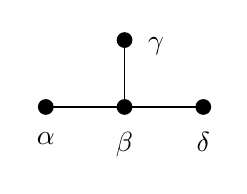
\begin{tikzpicture}
                \draw (1,0) to (2,0);
                \draw (2,0) to (2,0.85);
                \draw (2,0) to (3,0);
                \fill (1,0) circle (1mm);
                \fill (2,0) circle (1mm);
                \fill (2,0.85) circle (1mm);
                \fill (3,0) circle (1mm);
                \draw[below] (1,-0.2) node{$\alpha$};
                \draw[below] (2,-0.2) node{$\beta$};
                \draw[below] (2.4,1) node{$\gamma$};
                \draw[below] (3,-0.2) node{$\delta$};
               \end{tikzpicture}}
\end{figure}

We label $\Psi(G)^{+}$ in the following. The corresponding negative roos are defined accordingly. Note that Roots 1, 2, 3, 4 correspond to $\alpha$, $\gamma$, $\delta$, $\beta$ respectively.
\begin{table}[!h]
\begin{center}
\scalebox{0.7}{
\begin{tabular}{cccccc}
\rootsD{1}{0}{1}{0}{0}&\rootsD{2}{1}{0}{0}{0}&\rootsD{3}{0}{0}{0}{1}&\rootsD{4}{0}{0}{1}{0}&\rootsD{5}{0}{1}{1}{0}&\rootsD{6}{1}{0}{1}{0}\\
\rootsD{7}{0}{0}{1}{1}&\rootsD{8}{1}{1}{1}{0}&\rootsD{9}{0}{1}{1}{1}&\rootsD{10}{1}{0}{1}{1}&\rootsD{11}{1}{1}{1}{1}&\rootsD{12}{1}{1}{2}{1}\\
\end{tabular}
}
\end{center}
\end{table}   
Let
$\lambda:=(\alpha+2\beta+\gamma+\delta)^{\vee}=\alpha^{\vee}+2\beta^{\vee}+\gamma^{\vee}+\delta^{\vee}$. 
Then 
$
P_\lambda=\langle T, U_{\zeta}\mid \zeta\in \Psi(G)^{+}\cup \{-1,-2,-3\} \rangle,
L_\lambda=\langle T, U_{\zeta}\mid \zeta\in \{\pm 1,\pm 2,\pm 3\} \rangle,
R_u(P_\lambda)=\langle U_{\zeta} \mid \zeta \in \Psi(G)^{+}\backslash \{1, 2, 3\} \rangle.
$
Let $a\in k\backslash k^2$. Pick $b\in k^{*}$ with $b^3=1$ and $b\neq 1$. Let $v(\sqrt a):=\epsilon_{4}(\sqrt a)\epsilon_{11}(\sqrt a)\in R_u(P_\lambda)(\overline k)$. Define
\begin{equation*}
H:=v(\sqrt a)\cdot\langle n_\alpha n_\gamma n_\delta, \; (\alpha+\gamma+\delta)^{\vee}(b) \rangle.
\end{equation*}
Here is our first main result in this section.
\begin{prop}\label{firstmain}
$H$ is $k$-defined. Moreover, $H$ is $G$-cr but not $G$-cr over $k$. 
\end{prop}
\begin{proof}
First, we have 
$
(n_\alpha n_\gamma n_\delta) \cdot (\beta) = (n_\alpha n_\gamma n_\delta) \cdot 4 = 11, \;
(n_\alpha n_\gamma n_\delta) \cdot 11 = 4.
$
Using this and the commutation relations~\cite[Lem.~32.5 and Prop.~33.3]{Humphreys-book1}, we obtain
\begin{equation*}
v(\sqrt a)\cdot (n_{\alpha} n_\gamma n_\delta)=(n_\alpha n_\gamma n_\delta) \epsilon_{12}(a).
\end{equation*}
Since $\langle 4, (\alpha+\gamma+\delta)^{\vee}\rangle=-3$, $\langle 11, (\alpha+\gamma+\delta)^{\vee}\rangle=3$, and $b^3=1$, $v(\sqrt a)$ commutes with $(\alpha+\gamma+\delta)^{\vee}(b)$. Now it is clear that $H$ is $k$-defined (since it is generated by $k$-points). 

Now we show that $H$ is $G$-cr. It is sufficient to show that $H':=v(\sqrt a)^{-1}\cdot H=\langle n_\alpha n_\gamma n_\delta,\; (\alpha+\gamma+\delta)^{\vee}(b)$ is $G$-cr since it is $G$-conjugate to $H$. Since $H'$ is contained in $L_\lambda$, by Proposition~\ref{G-cr-L-cr} it is enough to show that $H'$ is $L_\lambda$-cr. By inspection, $H'$ is $L_\lambda$-ir (this is easy since $L_\lambda=L_\alpha\times L_\gamma\times L_\delta=A_1\times A_1 \times A_1$). 


Next, we show that $H$ is not $G$-cr over $k$. Suppose the contrary. Clearly $H$ is contained in $P_\lambda$ that is $k$-defined. Then there exists a $k$-defined Levi subgroup of $P_\lambda$ containing $H$. Then by~\cite[Lem.~2.5(\rmnum{3})]{Bate-uniform-TransAMS} there exists $u\in R_u(P_\lambda)(k)$ such that $H$ is contained in $u\cdot L_\lambda$. Thus $n_\alpha n_\gamma n_\delta \epsilon_{12}(a) < u\cdot L_\lambda$. So $u^{-1}\cdot (n_\alpha n_\gamma n_\delta \epsilon_{12}(a)) < L_{\lambda}$. By~\cite[Prop.~8.2.1]{Springer-book}, we set
$
u:=\prod_{\zeta\in \Psi(R_u(P_\lambda))}\epsilon_\zeta(x_\zeta).
$
Using the labelling of the positive roots above, we have $\Psi(R_u(P_\lambda))=\{4,\cdots 12\}$. We compute how $n_\alpha n_\gamma n_\delta$ acts on $\Psi(R_u(P_\lambda))$: 
\begin{equation}\label{perm}
n_\alpha n_\gamma n_\delta = (4\;11) (5\;10) (6\;9) (7\;8) (12). 
\end{equation}
Using this and the commutation relations,
\begin{alignat*}{2}
u^{-1}\cdot (n_\alpha n_\gamma n_\delta \epsilon_{12}(a))
=&n_\alpha n_\gamma n_\delta \epsilon_4(x_4+x_{11})\epsilon_{5}(x_5+x_{10})\epsilon_{6}(x_6+x_9)\epsilon_{7}(x_{7}+x_{8})\\
&\epsilon_{8}(x_7+x_8)\epsilon_{9}(x_6+x_{9})\epsilon_{10}(x_5+x_{10})\epsilon_{11}(x_4+x_{11})\\
&\epsilon_{12}(x_{4}^2+x_{5}^2+x_{6}^2+x_{7}^2 +a).
\end{alignat*}
Thus if $u^{-1}\cdot (n_\alpha\sigma \epsilon_{\alpha+2\beta+\gamma+\delta}(a)) < L_{\lambda}$ we must have
\begin{equation*}
x_4=x_{11},\; x_5=x_{10},\; x_{6}=x_{9},\; x_7=x_8,\; x_{4}^2+ x_{5}^2+x_{6}^2+x_{7}^2 +a=0.
\end{equation*}
The last equation gives $(x_4+x_5+x_6+x_7)^2=a$. This is impossible since $a\notin k^2$. We are done. 
\end{proof}

\begin{rem}\label{D4nonsep}
From the computations above we see that the curve $C(x):=\{\epsilon_{4}(x)\epsilon_{11}(x)\mid x\in \overline k\}$ is not contained in $C_G(H)$, but the corresponding element in $\textup{Lie}(G)$, that is, $e_4+e_{11}$ is contained in $\mathfrak{c}_{\mathfrak{g}}(H)$. Then the argument in the proof of~\cite[Prop.~3.3]{Uchiyama-Separability-JAlgebra} shows that $\textup{Dim}(C_G(H))$ is strictly smaller than $\textup{Dim}(\mathfrak{c}_{\mathfrak{g}}(H))$. So $H$ is non-separable in $G$. 
In fact, combining~\cite[Thm.~1.5]{Bate-cocharacter-Arx} and~\cite[Thm.~9.3]{Bate-cocharacter-Arx} we have that if a $k$-subgroup $H$ of $G$ is separable in $G$ and $H$ is $G$-cr, then it is $G$-cr over $k$. 
\end{rem}

\vspace{5mm}
Now we move on to the second main result in this section. We use the same $k$, $a$, $b$, $G$, and, $\lambda$ as above. Let $v(\sqrt a):=\epsilon_{-11}(\sqrt a)\epsilon_{-4}(\sqrt a)$. Let
\begin{equation*}
K:=v(\sqrt a)\cdot \langle n_{\alpha} n_{\gamma} n_{\delta},\; (\alpha+\gamma+\delta)^{\vee}(b)\rangle=\langle n_\alpha n_\gamma n_\delta \epsilon_{-12}(a), \;  (\alpha+\gamma+\delta)^{\vee}(b)\rangle. 
\end{equation*}
Define
\begin{equation*}
H:=\langle K, \; \epsilon_{5}(1) \rangle.
\end{equation*}

\begin{prop}\label{secondmain}
$H$ is $k$-defined. Moreover, $H$ is $G$-ir over $k$ but not $G$-cr. 
\end{prop}
\begin{proof}
$H$ is clearly $k$-defined. First, we show that $H$ is $G$-ir over $k$. Note that
\begin{equation*}
v(\sqrt a)^{-1}\cdot H = \langle n_\alpha n_\gamma n_\delta, \; (\alpha+\gamma+\delta)^{\vee}(b),\; \epsilon_{5}(1)\epsilon_{1}(\sqrt a)\rangle.
\end{equation*}
Thus we see that $v(\sqrt a)^{-1}\cdot H$ is contained in $P_\lambda$. So $H$ is contained in $v(\sqrt a)\cdot P_\lambda$. 

\begin{lem}\label{uniquepara}
$v(\sqrt a)\cdot P_\lambda$ is the unique proper parabolic subgroup of $G$ containing $H$.
\end{lem}
\begin{proof}
Suppose that $P_\mu$ is a proper parabolic subgroup of $G$ containing $v(\sqrt a)^{-1}\cdot H$. In the proof of Proposition~\ref{firstmain} we have shown that $M:=\langle n_\alpha n_\gamma n_\delta, (\alpha+\gamma+\delta)^{\vee}(b)\rangle$ is $G$-cr. Then there exists a Levi subgroup $L$ of $P_\mu$ containing $M$ since $M$ is contained in $P_\mu$. Since Levi subgroups of $P_\mu$ are $R_u(P_\mu)$-conjugate by~\cite[Lem.~2.5(\rmnum{3})]{Bate-uniform-TransAMS}, without loss, we set $L:=L_\mu$. Then $M<L_\mu=C_G(\mu(\overline k^*))$, so $\mu(\overline k^*)$ centralizes $M$. Recall that by~\cite[Thm.~13.4.2]{Springer-book}, $C_{R_u(P_\lambda)}(M)^{\circ}\times C_{L_\lambda}(M)^{\circ}\times C_{R_u(P_\lambda^{-})}(M)^{\circ}$ is an open set of $C_G(M)^{\circ}$ where $P_\lambda^{-}$ is the opposite of $P_\lambda$ containing $L_\lambda$.  
\begin{lem}\label{centralizerofM}
$C_G(M)^{\circ}=G_{12}$.
\end{lem}
\begin{proof}
First of all, from Equation~(\ref{perm}) we see that $G_{12}$ is contained in $C_G(n_\alpha n_\gamma n_\delta)$. Since $\langle 12, (\alpha+\gamma+\delta)^{\vee} \rangle=0$, $G_{12}$ is also contained in $C_G((\alpha+\gamma+\delta)^{\vee}(\overline k^*))$. So $G_{12}$ is contained in $C_G(M)$. Set $u:=\prod_{i\in \Psi(R_u(P_\lambda))}\epsilon_{i}(x_i)$ for some $x_i \in \overline k$. Using Equation (\ref{perm}) and the commutation relations, we obtain
\begin{alignat*}{2}
(n_\alpha n_\gamma n_\delta)\cdot u =& \epsilon_{4}(x_{11})\epsilon_{5}(x_{10})\epsilon_{6}(x_9)\epsilon_7(x_{8})\epsilon_8(x_{7})\epsilon_9(x_6)\epsilon_{10}(x_{5})\epsilon_{11}(x_4)\\
&\epsilon_{12}(x_4 x_{11}+x_5 x_{10} +x_6 x_9+ x_7 x_8+ x_{12}). 
\end{alignat*}
So, if $u\in C_{R_u(P_\lambda)}(n_\alpha n_\gamma n_\delta)$ we must have
$x_4=x_{11}, \; x_5=x_{10},\; x_{6}=x_{9},\; x_7=x_8$, and $x_4 x_{11}+x_5 x_{10} +x_6 x_9+ x_7 x_8=0$. But $\langle \zeta, (\alpha+\gamma+\delta)^{\vee}\rangle=-1$ for $\zeta=\{5, 6, 7\}$, so $x_5=x_6=x_7=0$ for $u\in C_{R_u(P_\lambda)}(M)$. Then 
\begin{equation*}
(n_\alpha n_\gamma n_\delta)\cdot u = \epsilon_4(x_4)\epsilon_{11}(x_4)\epsilon_{12}(x_4^2+x_{12}).
\end{equation*}
So we must have $x_4^2=0$ if $u\in C_{R_u(P_\lambda)}(M)$. Thus we conclude that $C_{R_u(P_\lambda)}(M)=U_{12}$. Similarly, we can show that $C_{R_u(P_{\lambda}^{-})}(M)=U_{-12}$. A direct computation shows that $C_{L_\lambda}(M) < T$ and $C_T(n_\alpha n_\gamma n_\delta)=(\alpha+2\beta+\gamma+\delta)^{\vee}(\overline k^*)<G_{12}$. We are done.
\end{proof}
Since $\mu(\overline k^*)$ centralizes $M$, Lemma~\ref{centralizerofM} yields $\mu(\overline k^*)<G_{12}$. Then we can set $\mu:=g\cdot (\alpha+2\beta+\gamma+\delta)^{\vee}$ for some $g\in G_{12}$. By the Bruhat decomposition, $g$ is one of the following forms:
\begin{alignat*}{2}
&(1)\;g=(\alpha+2\beta+\gamma+\delta)^{\vee}(s)\epsilon_{12}(x_1),\\
&(2)\;g=\epsilon_{12}(x_1)n_{12}(\alpha+2\beta+\gamma+\delta)^{\vee}(s)\epsilon_{12}(x_2)\\
&\textup{for some } x_1, x_2\in \overline k, s\in \overline k^*.
\end{alignat*}
We rule out the second case. Suppose $g$ is of the second form. Note that $\epsilon_{5}(1)\epsilon_{1}(\sqrt a)\in v(\sqrt a)^{-1}\cdot H< P_\mu$. 
But $P_\mu=P_{g\cdot (\alpha+2\beta+\gamma+\delta)^{\vee}}=g\cdot P_{(\alpha+2\beta+\gamma+\delta)^{\vee}}$. So it is enough to show that $g^{-1}\cdot (\epsilon_{5}(1)\epsilon_{1}(\sqrt a))\notin P_{(\alpha+2\beta+\gamma+\delta)^{\vee}}$. Since $U_{12}$ and $(\alpha+2\beta+\gamma+\delta)(\overline k^*)$ are contained in $P_{(\alpha+2\beta+\gamma+\delta)^{\vee}}$ we can assume $g=n_{12}$. We have
\begin{equation*}
n_{12}=n_\alpha n_\beta n_\alpha n_\gamma n_\beta n_\alpha n_\delta n_\beta n_\alpha n_\gamma n_\beta n_\delta \textup{ (the longest element in the Weyl group of $D_4$)}.
\end{equation*}
Using this, we can compute how $n_{12}$ acts on each root subgroup of $G$. In particular $n_{12}^{-1}\cdot U_{5}=U_{-5}$ and $n_{12}^{-1}\cdot U_{1}= U_{-1}$. Thus
\begin{alignat*}{2}
n_{12}^{-1}\cdot (\epsilon_{5}(1)\epsilon_{1}(\sqrt a)) &= \epsilon_{-5}(1)\epsilon_{-1}(\sqrt a)\notin P_{(\alpha+2\beta+\gamma+\delta)^{\vee}}.
\end{alignat*}
So $g$ must be of the first form. Then $g\in P_\lambda$. Thus $P_\mu=P_{g\cdot \lambda}=g\cdot P_\lambda=P_\lambda$. We are done.
\end{proof}

\begin{lem}\label{nonkdefined}
$v(\sqrt a)\cdot P_\lambda$ is not $k$-defined.
\end{lem}
\begin{proof}
Suppose the contrary. Since $P_\lambda$ is $k$-defined, $v(\sqrt a)\cdot P_\lambda$ is $G(k)$-conjugate to $P_\lambda$ by~\cite[Thm.~20.9]{Borel-AG-book}. Thus we can put $P_\lambda=g v(\sqrt a)\cdot P_\lambda$ for some $g\in G(k)$. So $g v(\sqrt a)\in P_\lambda$ since parabolic subgroups are self-normalizing. Then $g=pv(\sqrt a)^{-1}$ for some $p\in P_\lambda$. Thus $g$ is a $k$-point of $P_\lambda R_u(P_\lambda^{-})$. Then by the rational version of the Bruhat decomposition~\cite[Thm.~21.15]{Borel-AG-book}, there exists a unique $p'\in P_\lambda(k)$ and a unique $u'\in R_u(P_\lambda^{-})(k)$ such that $g=p' u'$. This is a contradiction since $v(\sqrt a)\notin R_u(P_\lambda^{-})(k)$. 
\end{proof} 
Now Lemmas~\ref{uniquepara},~\ref{nonkdefined} show that $H$ is $G$-ir over $k$. 

\begin{lem}\label{nonG-cr}
$H$ is not $G$-cr. 
\end{lem}
\begin{proof}
We had $C_G(M)^{\circ}=G_{12}$. Then $C_G(v(\sqrt a)^{-1}\cdot H)^{\circ}<G_{12}$ since $M<v(\sqrt a)^{-1}\cdot H$. Using the commutation relations, we see that $U_{12}< C_G(v(\sqrt a)^{-1}\cdot H)$. Note that $v(\sqrt a)^{-1}\cdot H$ contains $h:=\epsilon_{5}(1)\epsilon_{1}(\sqrt a)$ that does not commute with any non-trivial element of $U_{-12}$. Also, since $\langle 5, \lambda\rangle = 4$,  $h$ does not commute with any non-trivial element of $(\alpha+2\beta+\gamma+\delta)^{\vee}(\overline k^*)$.
Thus we conclude that $C_G(v(\sqrt a)^{-1}\cdot H)^{\circ}=U_{12}$. So $C_G(H)^{\circ}=v(\sqrt a)\cdot U_{12}$ which is unipotent. Then by the classical result of Borel-Tits~\cite[Prop.~3.1]{Borel-Tits-unipotent-invent}, we see that $C_G(H)^{\circ}$ is not $G$-cr.
Since $C_G(H)^{\circ}$ is a normal subgroup of $C_G(H)$, by~\cite[Ex.~5.20]{Bate-uniform-TransAMS}, $C_G(H)$ is not $G$-cr. Then by~\cite[Cor.~3.17]{Bate-geometric-Inventione}, $H$ is not $G$-cr. 
\end{proof}
\end{proof}



  
\section{Tits' center conjecture}
In~\cite{Tits-colloq}, Tits conjectured the following:
\begin{con}\label{centerconjecture}
Let $X$ be a spherical building. Let $Y$ be a convex contractible simplicial subcomplex of $X$. If $H$ is an automorphism group of $X$ stabilizing $Y$, then there exists a simplex of $Y$ fixed by $H$.   
\end{con}
This so-called center conjecture of Tits was proved by case-by-case analyses by Tits, M\"{u}hlherr, Leeb, and Ramos-Cuevas~\cite{Leeb-Ramos-TCC-GFA},~\cite{Muhlherr-Tits-TCC-JAlgebra},~\cite{Ramos-centerconj-Geo}. Recently uniform proof was given in~\cite{Weiss-center-Fourier}. In relation to the theory of complete reducibility, Serre showed~\cite{Serre-building}:
\begin{prop}\label{SerreContractible}
Let $G$ be a reductive $k$-group. Let $\Delta(G)$ be the building of $G$. If $H$ is not $G$-cr, then the fixed point subcomplex $\Delta(G)^H$ is  convex and contractible. 
\end{prop}
We identify the set of proper $k$-parabolic subgroups of $G$ with $\Delta(G)$ in the usual sense of Tits~\cite{Tits-book}. Note that for a subgroup $H$ of $G$, $N_G(H)(k)$ induces an automorphism group of $\Delta(G)$ stabilizing $\Delta(G)^H$. Thus, combining the center conjecture with Proposition~\ref{SerreContractible} we obtain
\begin{prop}\label{normalizer}
If a subgroup $H$ of $G$ is not $G$-cr over $k$, then there exists a proper $k$-parabolic subgroup of $G$ containing $H$ and $N_G(H)(k)$. 
\end{prop}
Proposition~\ref{normalizer} was an essential tool to prove various theoretical results on complete reducibility over nonperfect $k$ in~\cite{Uchiyama-Nonperfectopenproblem-pre} and~\cite{Uchiyama-Nonperfect-pre}. We have asked the following in~\cite[Rem.~6.5]{Uchiyama-Nonperfectopenproblem-pre}:
\begin{question}\label{centralizerQ}
If $H<G$ is not $G$-cr over $k$, then does there exist a proper $k$-parabolic subgroup of $G$ containing $HC_G(H)$?
\end{question}
The answer is yes if $C_G(H)$ is $k$-defined (or $k$ is perfect). Since in that case the set of $k$ points are dense in $C_G(H)$ (since we assume $k=k_s$) and the result follows from Proposition~\ref{normalizer}. The main result in this section is to present a counterexample to Question~\ref{centralizerQ} when $k$ is nonperfect. 
\begin{thm}\label{centralizerA}
Let $k$ be nonperfect of characteristic $2$. Let $G$ be simple of type $D_4$. Then there exists a non-abelian $k$-subgroup $H$ of $G$ such that $H$ is not $G$-cr over $k$ but $C_G(H)$ is not contained in any proper $k$-parabolic subgroup of $G$. 
\end{thm}
\begin{rem}
Borel-Tits~\cite[Rem.~2.8]{Borel-Tits-unipotent-invent} mentioned that if $k$ is nonperfect of characteristic $2$ and $[k:k^2]>2$, there exists a $k$-plongeable unipotent element $u$ in $G$ of type $D_4$ such that $C_G(u)$ is not contained in any proper $k$-parabolic subgroup of $G$ (with no proof). Note that such $u$ generates a (cyclic) subgroup of $G$ that is not $G$-cr over $k$. (Recall that a unipotent element is called $k$-plongeable if it can be embedded in the unipotent radical of a proper $k$-parabolic subgroup of $G$~\cite{Borel-Tits-unipotent-invent}.) Theorem~\ref{centralizerA} is a nonabelian version of Borel-Tits' result. Also the assumption $[k:k^2]>2$ is not necessary here. 
\end{rem}
\begin{proof}
We keep the same notation from the previous section. Set $n:=n_\alpha n_\gamma n_\delta$,  $t:=(\alpha+\gamma+\delta)^{\vee}(b)$, and $v(\sqrt a):=\epsilon_4(\sqrt a)\epsilon_{11}(\sqrt a)$. Let $H:=\langle n_\alpha n_\gamma n_\delta \epsilon_{12}(a), (\alpha+\gamma+\delta)^{\vee}(b) \rangle$.  Then $H$ is not $G$-cr over $k$. 
We have $H':=v(\sqrt a)^{-1}\cdot H = \langle n, t \rangle$. It is clear that $C_G(H')>G_{12}$. Thus $\langle n, t, G_{12} \rangle < H'C_G(H')$. By running a similar argument as in the proof of Lemma~\ref{uniquepara} in the previous section, we find that the only proper parabolic subgroup of $G$ containing $\langle n, t, U_{12} \rangle$ is $P_{(\alpha+2\beta+\gamma+\delta)^{\vee}}$ (since $n_{12}\cdot 12 = -12$). Clearly $P_{(\alpha+2\beta+\gamma+\delta)^{\vee}}$ does not contain $G_{12}$. Therefore there is no proper parabolic subgroup of $G$ containing $H'C_G(H')$. Thus there is no proper parabolic subgroup of $G$ containing $HC_G(H)$. 
\end{proof}


\section{G-cr vs $M$-cr (Proof of Theorem~\ref{G-cr-M-cr})}
From this section we assume $k$ is algebraically closed. Let $G$ be as in the hypothesis. Let $a, b\in k^{*}$ with $b^3=1$ and $b\neq 1$. Let $H':=\langle n_\alpha n_\gamma n_\delta, (\alpha+\gamma+\delta)^{\vee}(b) \rangle$. Let $v(a):=\epsilon_4(a)\epsilon_{11}(a)$. Define
\begin{equation*}
H:=v(a)\cdot H' = \langle n_\alpha n_\gamma n_\delta \epsilon_{12}(a^2), (\alpha+\gamma+\delta)^{\vee}(b)\rangle.  
\end{equation*}
Then $H$ is $G$-cr (by the same argument as in the previous section). Now let $M:=\langle G_{\alpha}, G_{\gamma}, G_{\delta}, G_{12}\rangle\cong A_1 A_1 A_1 A_1$. 
\begin{prop}
$H$ is not $M$-cr. 
\end{prop}
\begin{proof}
Let $\lambda:=(\alpha+2\beta+\gamma+\delta)^{\vee}$. Then $H<P_\lambda(M)=\langle T, G_{\alpha}, G_{\gamma}, G_{\delta}, U_{12}\rangle$. Let $c_\lambda: P_\lambda\rightarrow L_\lambda$ be the natural projection. Let $v:=(n_\alpha n_\gamma n_\delta \epsilon_{12}(a^2), (\alpha+\gamma+\delta)^{\vee}(b))$. We have
\begin{equation*}
c_\lambda(v)=\lim_{a\rightarrow 0}\lambda(a)\cdot (n_\alpha n_\gamma n_\delta \epsilon_{12}(a^2), (\alpha+\gamma+\delta)^{\vee}(b))= (n_\alpha n_\gamma n_\delta, (\alpha+\gamma+\delta)^{\vee}(b)).
\end{equation*}
We see that $v$ is not $R_u(P_\lambda(M))$-conjugate to $c_\lambda(v)$ since $R_u(P_\lambda (M))=U_{12}$ centralizes $n_\alpha n_\gamma n_\delta$. By Proposition~\ref{unipotentconjugate}, this shows that $H$ is not $M$-cr. 
\end{proof}
  



\section{K\"ulshammer's question (Proof of Theorem~\ref{thmKul})}
Let $d\geq 5$ be odd. Let $D_{2d}$ be the dihedral group of order $2d$. Let 
\begin{equation*}
\Gamma:=D_{2d}\times C_2 =\langle r, s, z\mid r^d=s^2=z^2=1, srs^{-1}=r^{-1}, [r,z]=[s,z]=1\rangle.
\end{equation*}
Let $\Gamma_2:=\langle s, z\rangle$ (a Sylow $2$-subgroup of $\Gamma$). Let $G$ be as in the hypothesis. Choose $a, b\in k^{*}$ with $b^d=1$ and $b\neq 1$. Let $n:=n_\alpha n_\gamma n_\delta$ and $t:=(\alpha+\gamma+\delta)^{\vee}(b)$. For each $a\in k$ define $\rho_a\in \textup{Hom}(\gamma, G)$ by
\begin{equation*}
\rho_a(r)=t, \; \rho_a(s)=n \epsilon_{12}(a), \; \rho_a(z)=\epsilon_{12}(1). 
\end{equation*}
An easy computation shows that this is well-defined. 
Let $u(\sqrt a)=\epsilon_{4}(\sqrt a)\epsilon_{11}(\sqrt a)$. Then $u(\sqrt a)\cdot n = n\epsilon_{12}(a)$ and $u(\sqrt a)\cdot \epsilon_{12}(1) = \epsilon_{12}(1)$. Thus $u(\sqrt a)\cdot (\rho_0\mid_{\Gamma_2})=\rho_a\mid_{\Gamma_2}$. So $\rho_a\mid_{\Gamma_2}$ are pairwise conjugate. 

Now suppose that $\rho_a$ is conjugate to $\rho_b$. Then there exists $g\in G$ such that $g\cdot \rho_a=\rho_b$. Since $\rho_a(r)=t$, we must have $g\in C_G(t)=TG_{12}$. So let $g=hm$ for some $h\in T$ and $m\in G_{12}$. Then we have
\begin{alignat*}{2}
hnh^{-1}(hm\epsilon_{12}(a)m^{-1}h^{-1})&= hnm\epsilon_{12}(a)m^{-1}h^{-1}\\
                                                                 &= hmn\epsilon_{12}(a)m^{-1}h^{-1}\\
                                                                 &= g\cdot \rho_{a}(s)\\
                                                                 &= \rho_b(s)\\
                                                                 &= n\epsilon_{12}(b).
\end{alignat*}
Note that $hnh^{-1}\in G_\alpha G_\gamma G_\delta$ and $hm\epsilon_{12}(a)m^{-1}h^{-1}\in G_{12}$. Since $[G_\alpha G_\gamma G_\delta, G_{12}]=1$, we have $G_\alpha G_\gamma G_\delta \cap G_{12}=1$. This implies $hnh^{-1}=n$. Now an easy computation shows $h\in G_{12}$. Thus $g=hm\in G_{12}$. Since $G_{12}$ is a simple group of type $A_1$, $(n\epsilon_{12}(a), \epsilon_{12}(1))$ cannot be $G_{12}$- conjugate to $(n\epsilon_{12}(b), \epsilon_{12}(1))$ if $a\neq b$. We are done.                                                                 

\section{Conjugacy classes (Proof of Theorem~\ref{conjugacy-counterexample})}

\begin{proof}
Let $G$ be as in the hypothesis. Let $\lambda:=(\alpha+2\beta+\gamma+\delta)^{\vee}$. Then $\Psi(R_u(P_\lambda))=\{4,\cdots, 12\}$. Using the commutation relations we have $Z(R_u(P_\lambda))=U_{12}$. Let $n:=n_\alpha n_\gamma n_\delta$. Pick $b\in k$ with $b^3=1$ and $b\neq 1$. Let $t:=(\alpha+\gamma+\delta)^{\vee}(b)$. Define $K:=\langle n, t, U_{12} \rangle$. 
By the same argument as that in the proof of~\cite[Lem.~5.1]{Uchiyama-Separability-JAlgebra} we obtain $C_{P_\lambda}(K)=C_{R_u(P_\lambda)}(K)$ (since $\langle 12, \lambda\rangle=2$). By a standard result there exists $n\in \mathbb{N}$ such that $Z=\langle z_1,\cdots, z_n \rangle$. Now let $M:=\langle L_\lambda, G_{12} \rangle$. Let ${\bf m}:=(n, t, z_1,\cdots, z_n)$ and set $N:=n+2$. Then by the similar argument to that in the proof of~\cite[Lem.~5.1]{Uchiyama-Separability-JAlgebra} yields that $G\cdot {\bf m}\cap P_\lambda(M)^N$ is an infinite union of $P_\lambda(M)$-conjugacy classes. (The crucial thing here is the existence of a curve that is tangent to $\mathfrak{c}_{\mathfrak{g}}(K)$ but not tangent to $C_G(K)$, in other words $K$ is nonseparable in $G$.) Now let $c_\lambda:P_\lambda\rightarrow L_\lambda$ be the canonical projection. Then $c_\lambda(n, t, z_1, \cdots, z_n)=(n,t)$. Since $K_0:=\langle n, t \rangle$ is $L$-ir as shown in the previous section, by~\cite[Prop.~3.5.2]{Stewart-thesis} we are done. 
\end{proof}


\documentclass{article}

\begin{document}

\section{Acknowledgements}

The author would like to thank B. J. Hiley, M. Hajtanian, and D. Nellist for their insightful conversations and support.

\end{document}
\bibliography{mybib}

\end{document}